\subsubsection{Flöde vid termisk jämvikt}

%To regerenate the figures use /code/pdesolver/generateWallFigApril.m
%with the argument /code/pdesolver/walldata.mat

\begin{figure}
\centering

\subfloat[Energiflöde en molnfri dag ut från insidan av en vägg med $0,5\mbox{m}$
tegel.]{
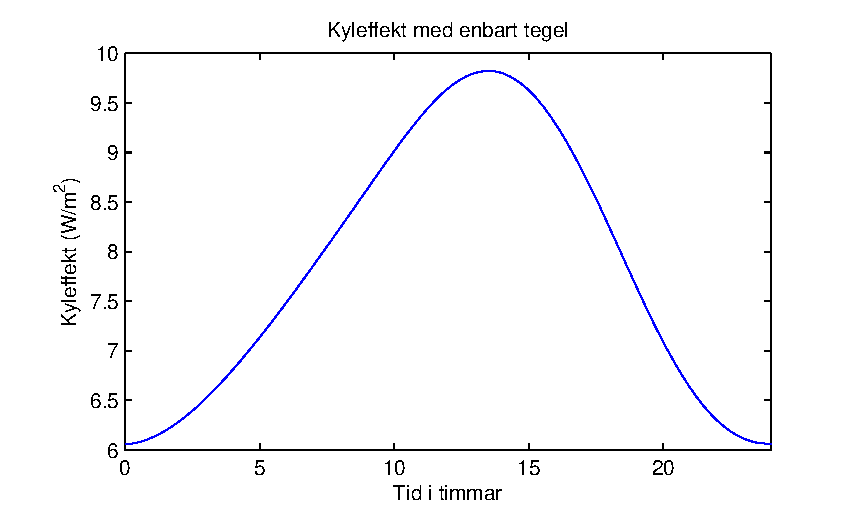
\includegraphics[width=6cm]{images/noinsulationapril.eps}
}\vspace{5mm}
\subfloat[Energiflöde en molnfri dag ut från insidan av en vägg med $0,5\mbox{m}$ tegel och
$1\mbox{dm}$ tilläggsisolering bestående av mineralull.]{
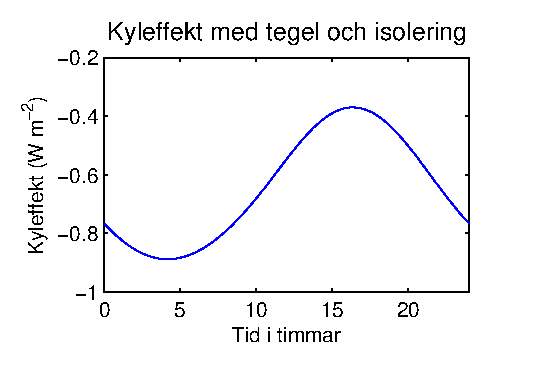
\includegraphics[width=6cm]{images/insulationapril.eps}}

\subfloat[Energiflöde en molnig dag ut från insidan av en vägg med $0,5\mbox{m}$.]{
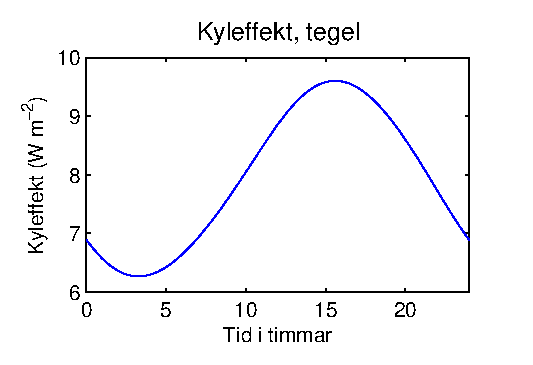
\includegraphics[width=6cm]{images/noinsulationcloud.eps}
}\vspace{5mm}
\subfloat[Energiflöde en molnig dag ut från insidan av en vägg med $0,5\mbox{m}$ tegel och
$1\mbox{dm}$ tilläggsisolering bestående av mineralull.]{
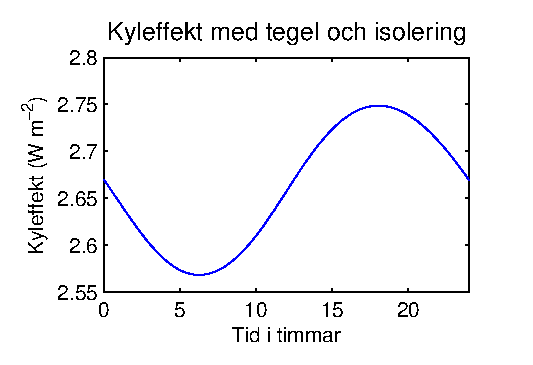
\includegraphics[width=6cm]{images/insulationcloud.eps}
}

\caption{Energiflödena är tagna från en fiktiv dag som skulle motsvara en molnfri
och en molnig
15 april 2011. Här har temperaturen varierat mellan 6 grader Celsius på natten och
9 grader Celsius på dagen. Beräkningen är genomförd med finita elementmetoden där
temperaturen på insidan av väggen satts till konstanta $\unit[20]{^\circ C}$.}
\end{figure}


\begin{figure}
\centering
\subfloat[Energiflöde en molnig decemberdag från insidan av en vägg med $0,5\mbox{m}$
tegel.]{
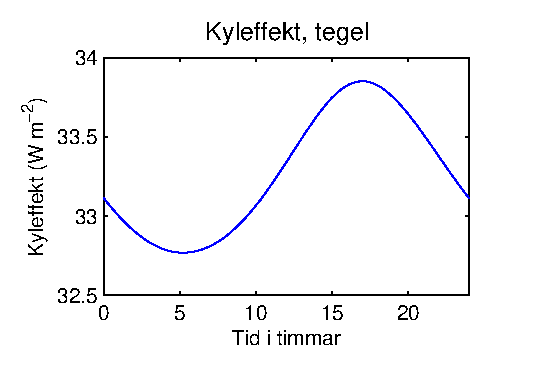
\includegraphics[width=6cm]{images/noinsulationdec.eps}
}
\vspace{5mm}
\subfloat[Energiflöde en molnig decemberdag från insidan av en vägg med
$0,5\mbox{m}$ tegel och $1\mbox{dm}$ tilläggsisolering bestående av mineralull.]{
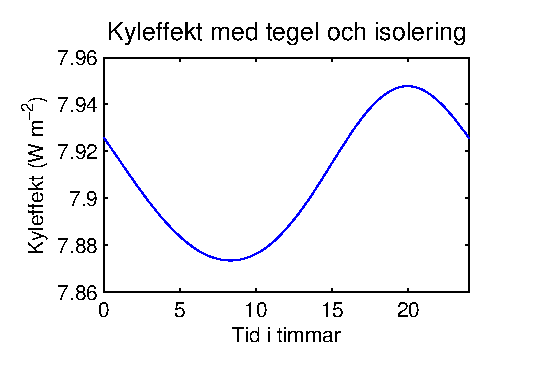
\includegraphics[width=6cm]{images/insulationdec.eps}
}
\caption{Ovanstående energiflöden är beräknade en molnig dag där
utomhus temperaturen går från $\unit[-5]{^\circ C}$ på dagen
till $\unit[-11]{^\circ C}$ på natten. Solinstrålningen denna dag är
räknad som $\unit[20]{\%}$ av vad den skulle varit den $31$ december $2011$.
Detta kan ses som ett extremfall på nyår för Göteborg och är då en övre
uppskattning på den energiåtgång fastigheten har vid denna årstid.
Konvektionskoefficienten har här satts till $h=35$ som motsvarar
$\unit[5]{m/s}$ paralellt med väggens yta. Beräkningarna är genomförda
genom att väggen approximerats som en stav och därefter behandlats med
finita elementmetoden.}
\end{figure}
